% Fig. 1 of the DSN paper: the robustness test and its two artifacts as five small graphs.
% Drawn at print size (7 in wide; 7 pt labels, 8 pt titles). Numbers follow the worked example of Section III-B.
% Build: pdflatex fig_problem_src.tex && mv fig_problem_src.pdf fig_problem.pdf
\documentclass[10pt]{standalone}
\pdfinfoomitdate=1 \pdftrailerid{}
\usepackage{amsmath}
\usepackage{tikz}
\usetikzlibrary{arrows.meta,decorations.pathreplacing}
\begin{document}
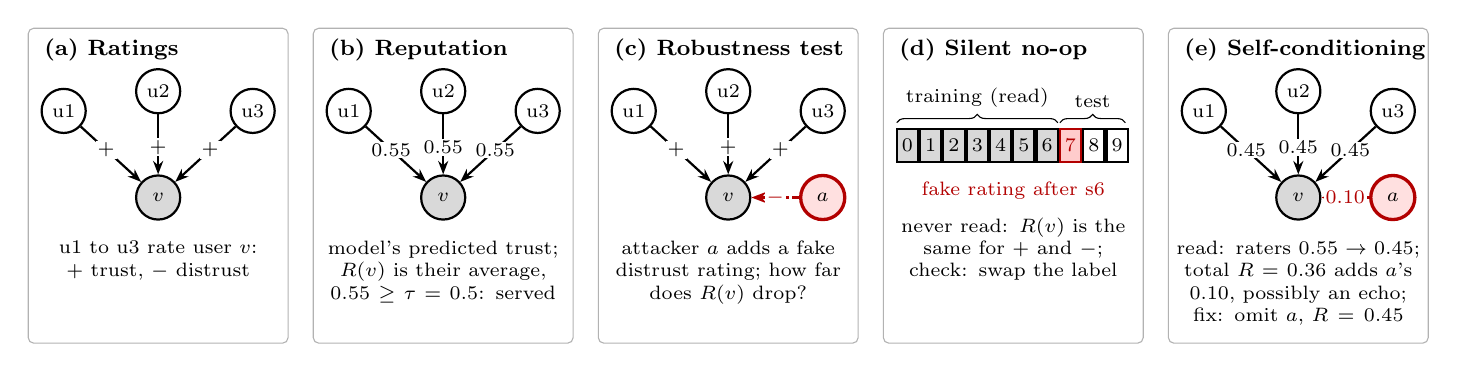
\begin{tikzpicture}[
  font=\scriptsize,
  user/.style={circle,draw,thick,minimum size=5.6mm,inner sep=0pt},
  tgt/.style={user,fill=black!15},
  atk/.style={user,draw=red!70!black,fill=red!12,very thick},
  rate/.style={-{Stealth[length=1.7mm]},thick},
  fake/.style={-{Stealth[length=1.9mm]},very thick,red!70!black,dash pattern=on 2.4pt off 1.4pt},
  lab/.style={fill=white,inner sep=0.7pt},
  ttl/.style={font=\footnotesize\bfseries,anchor=west},
  txt/.style={anchor=north,align=center,text width=3.2cm,inner sep=0pt},
]
\def\W{3.3}\def\H{4.0}\def\G{3.62}
\foreach \i in {0,...,4} \draw[black!30,rounded corners=2pt] (\i*\G,0) rectangle ++(\W,\H);
% Three raters u1..u3 and the target v at panel offset #1; edges labeled #1.
\newcommand{\raters}[1]{%
  \node[user] (u1) at (#1+0.45,2.95) {u1};
  \node[user] (u2) at (#1+1.65,3.2) {u2};
  \node[user] (u3) at (#1+2.85,2.95) {u3};
  \node[tgt] (v) at (#1+1.65,1.85) {$v$};}
\newcommand{\redges}[1]{%
  \draw[rate] (u1) -- node[lab,pos=0.42] {#1} (v);
  \draw[rate] (u2) -- node[lab,pos=0.55] {#1} (v);
  \draw[rate] (u3) -- node[lab,pos=0.42] {#1} (v);}

% (a) Ratings
\node[ttl] at (0.08,3.72) {(a) Ratings};
\raters{0}\redges{$+$}
\node[txt] at (1.65,1.3) {u1 to u3 rate user $v$:\\ $+$ trust, $-$ distrust};

% (b) Reputation
\node[ttl] at (\G+0.08,3.72) {(b) Reputation};
\raters{\G}\redges{0.55}
\node[txt] at (\G+1.65,1.3) {model's predicted trust;\\ $R(v)$ is their average,\\ $0.55\ge\tau=0.5$: served};

% (c) Robustness test
\node[ttl] at (2*\G+0.08,3.72) {(c) Robustness test};
\raters{2*\G}\redges{$+$}
\node[atk] (a) at (2*\G+2.85,1.85) {$a$};
\draw[fake] (a) -- node[lab,text=red!70!black] {$-$} (v);
\node[txt] at (2*\G+1.65,1.3) {attacker $a$ adds a fake\\ distrust rating; how far\\ does $R(v)$ drop?};

% (d) Silent no-op: ten snapshots, the model reads s0..s6, the fake rating lands in s7
\node[ttl] at (3*\G+0.08,3.72) {(d) Silent no-op};
\foreach \k in {0,...,9} {
  \ifnum\k<7 \def\fc{black!15}\def\dc{black}\else\def\fc{white}\def\dc{black}\fi
  \ifnum\k=7 \def\fc{red!20}\def\dc{red!70!black}\fi
  \draw[thick,draw=\dc,fill=\fc] (3*\G+0.17+\k*0.296,2.3) rectangle ++(0.27,0.42);
  \node[text=\dc] at (3*\G+0.305+\k*0.296,2.51) {\k};
}
\draw[decorate,decoration={brace,amplitude=3pt}] (3*\G+0.17,2.8) -- (3*\G+2.216,2.8)
  node[midway,above=2pt] {training (read)};
\draw[decorate,decoration={brace,amplitude=3pt}] (3*\G+2.242,2.8) -- (3*\G+3.074,2.8)
  node[midway,above=2pt] {test};
\node[txt,text=red!70!black] at (3*\G+1.65,2.05) {fake rating after s6};
\node[txt] at (3*\G+1.65,1.6) {never read: $R(v)$ is the\\ same for $+$ and $-$;\\ check: swap the label};

% (e) Self-conditioning: in-window, raters drop to 0.45, the attacker's own prediction is 0.10
\node[ttl] at (4*\G+0.08,3.72) {(e) Self-conditioning};
\raters{4*\G}\redges{0.45}
\node[atk] (a) at (4*\G+2.85,1.85) {$a$};
\draw[fake] (a) -- node[lab,text=red!70!black] {0.10} (v);
\node[txt] at (4*\G+1.65,1.3) {read: raters $0.55\to0.45$;\\ total $R=0.36$ adds $a$'s\\ 0.10, possibly an echo;\\ fix: omit $a$, $R=0.45$};
\end{tikzpicture}
\end{document}
